\section{ART工作原理}
在ART中,APK在安装的时候,安装服务PackageManagerService会通过守护进程installd调用工具dex2oat对打包在APK里面包含有Dex字节码进翻译。这个翻译器实际上就是基于LLVM架构实现的一个编译器,它的前端是一个Dex语法分析器。翻译后得到的是一个ELF格式的oat文件,这个oat文件以.odex后缀结束,并且保存在/data/dalvik-cache目录中。关于ART的工作原理主要是下面3个方面:

1. 在Android系统启动过程中创建的Zygote进程利用ART运行时导出的Java虚拟机接口创建ART虚拟机

2. APK在安装的时候,打包在里面的classes.dex文件会被工具dex2oat翻译成本地机器指令,最终得到一个ELF格式的oat文件

3. APK运行时,上述生成的oat文件会被加载到内存中,并且ART虚拟机可以通过里面的oatdata和oatexec段找到任意一个类的方法对应的本地机器指令来执行

\subsection{ART虚拟机}
如图~\ref{fig:artvm},ART运行时实现了一套完全兼容Java虚拟机的接口,在Android系统中,Davik虚拟机实现在libdvm.so中,ART虚拟机实现在libart.so中。Android系统还提供了一个系统属性persist.sys.dalvik.vm.lib,它的值要么等于libdvm.so,要么等于libart.so。当等于libdvm.so时,就表示当前用的是Dalvik虚拟机,而当等于libart.so时,就表示当前用的是ART虚拟机。
\begin{figure}[hbpt]
\centering
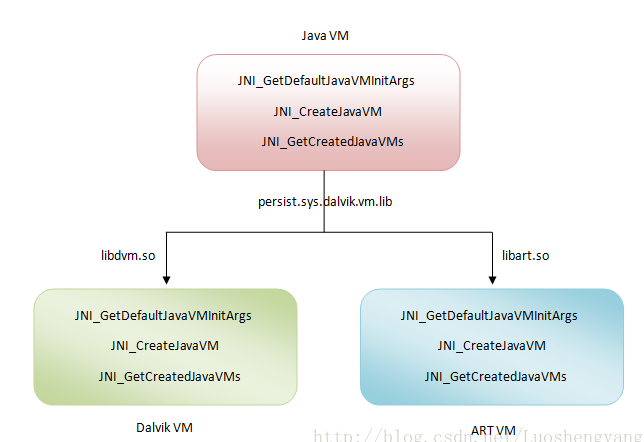
\includegraphics[width=\textwidth]{img/artvm.png}
\caption{Dalvik VM、ART VM与Java VM的关系}
\label{fig:artvm}
\end{figure}

Android系统在启动的时候,会创建一个Zygote进程,充当应用程序进程孵化器。Zygote进程在启动的过程中,又会创建一个Dalvik虚拟机。Zygote进程中的Dalvik虚拟机是从AndroidRutime::start这个函数开始创建的,这个函数定义在文件frameworks/base/core/jni/AndroidRuntime.cpp中,start函数的主要功能是:
       
创建一个JniInvocation实例,并且调用它的成员函数init来初始化JNI环境,init首先是读取系统属性persist.sys.dalvik.vm.lib的值,根据系统属性persist.sys.dalvik.vm.lib来初始化Dalvik虚拟机或者ART虚拟机环境

调用AndroidRutime类的成员函数startVm来创建一个虚拟机及其对应的JNI接口,startVm调用函数JNI\_CreateJavaVM创建一个JavaVM接口和一个JNIEnv接口

有了上述的JavaVM接口和JNIEnv接口之后,就可以在Zygote进程中加载指定的class
\subsection{dex到oat}
\begin{figure}[hbpt]
\centering
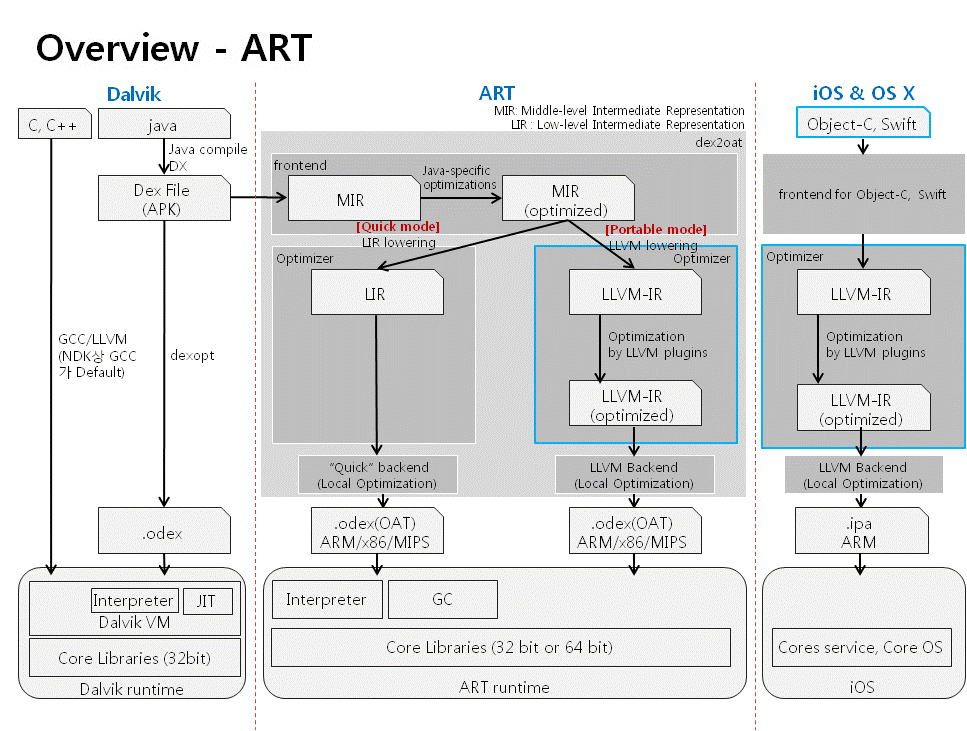
\includegraphics[width=\textwidth]{img/art-overview.png}
\caption{ART-Overview.}
\label{fig:art:overview}
\end{figure}
图~\ref{fig:art:overview}是ART的概览图,由图中描述dex文件转换成MIR,对MIR做优化,再由MIR转换成LIR,由MIR到LIR有两种形式:quick和portable,portable则是指转换为llvm IR,quick mode对应目录/art/compiler/dex/quick,portable对应目录/art/compiler/dex/portable,接着对LIR做优化,最后转化为oat格式文件。看了art目录下的代码,art编译代码的流程大致是:

1.从dex文件中提取类和方法并把方法变为为MIR: /art/compiler/dex/frontend.cc,frontend.cc文件中一个关键的类是CompileMethod,用于编译dex方法,调用MIRGraph类生成MIR
 
2.优化MIR: /art/compiler/dex/mir\_optimization.cc

3.MIR到llvm IR: /art/compiler/dex/portable/mir\_to\_gbc.cc

4.生成机器代码: /art/compiler/llvm/compiler\_llvm.cc

5.写入oat文件: /art/compiler/oat\_writer.cc

中间表示分为两种,MIR(middle-level intermediate representation)与LIR(low-level intermediate representation)。 MIR与LIR节点各自形成链表,分别被组织在BasicBlock与ConpilationUnit中。 编译流程是: 0、创建CompilationUnit对象来存放一次编译中需要的信息; 1、将dex文件中的Dalvik字节码解码为DecodedInstruction,并创建对应的MIR节点; 2、定位基本块的边界,并创建相应的BasicBlock对象,将MIR塞进去; 3、确定控制流关系,将基本块连接起来构成控制流图(CFG),并添加恢复解释器状态和异常处理用的基本块; 4、将基本块都加到CompilationUnit里去; 5、将MIR转换为LIR(带有局部优化和全局优化) 6、从LIR生成机器码。\url{http://source.android.com/tech/dalvik/index.html}中关于Dalvik虚拟机的指令集和dex文件格式的介绍,结合mir\_graph中的代码,转换为MIR的过程与这个网站上给出的bytecode set一致。mir到lir的转换则是遍历mir graph,每次处理一个基本块,替换基本块内的内容。

\subsection{oat执行}
ART运行时提供了一个OatFile类,通过调用它的静态成员函数Open可以在本进程中加载OAT文件,这个函数定义在文件art/runtime/oat\_file.cc中,
\begin{lstlisting}
OatFile* OatFile::Open(const std::string& filename,
                       const std::string& location,
                       byte* requested_base,
                       bool executable,
                       std::string* error_msg) {
  .............

}
\end{lstlisting}
参数filename和location指向要加载的OAT文件,参数requested\_base是一个可选参数,用来描述要加载的OAT文件里面的oatdata段要加载的位置,参数executable表示要加载的OAT是不是应用程序的主执行文件。一般来说,一个应用程序只有一个classes.dex文件, 这个classes.dex文件经过编译后,就得到一个OAT主执行文件。不过,应用程序也可以在运行时动态加载DEX文件。这些动态加载的DEX文件在加载的时候同样会被翻译成OAT再运行,就不属于主执行文件了。

ART运行时利用LLVM编译框架将DEX字节码翻译成本地机器指令,这些生成的机器指令就保存在ELF文件格式的OAT文件的oatexec段中.ART运行时会为每一个类方法都生成一系列的本地机器指令,这些本地机器指令不是孤立存在的,因为它们可能需要其它的函数来完成自己的功能。这要求Backend为类方法生成本地机器指令时,要处理调用其它模块提供的函数的问题。ART运行时支持两种类型的Backend:Portable和Quick。

Portable类型的Backend通过集成在LLVM编译框架里面的一个称为MCLinker的链接器来生成本地机器指令。这些OAT文件要通过系统的动态链接器提供的dlopen函数来加载。函数dlopen在加载OAT文件的时候,会通过重定位技术来处理好它与其它模块的依赖关系,使得它能够调用其它模块提供的接口。

Quick类型的Backend生成的本地机器指令用另外一种方式来处理依赖模块之间的依赖关系,ART运行时会在每一个线程的TLS(线程本地区域)提供一个函数表,Quick类型的Backend生成的本地机器指令通过引用这个函数表来调用其它模块的函数。也就是说,Quick类型的Backend生成的本地机器指令要依赖于ART运运时提供的函数表,这使得Quick类型的Backend生成的OAT文件在加载时不需要重定位,因此就不需要通过系统的动态链接器提供的dlopen函数来加载。由于省去重定位这个操作,Quick类型的Backend生成的OAT文件在加载时就会更快,这也是称为Quick的缘由。

如果在编译ART运行时时,定义了宏ART\_USE\_PORTABLE\_COMPILER,那么就表示要使用Portable类型的Backend来生成OAT文件,否则就使用Quick类型的Backend来生成OAT文件。Open函数的实现过程:

1. 如果编译时指定了ART\_USE\_PORTABLE\_COMPILER宏,并且参数executable为true,那么就通过OatFile类的静态成员函数OpenDlopen来加载指定的OAT文件。OatFile类的静态成员函数OpenDlopen直接通过动态链接器提供的dlopen函数来加载OAT文件。

2. 其余情况下,通过OatFile类的静态成员函数OpenElfFile来加载指定的OAT文件。这种方式是按照ELF文件格式来解析要加载的OAT文件的,并且根据解析获得的信息将OAT里面相应的段加载到内存中来。

OatFile类的成员函数Dlopen首先是通过动态链接器提供的dlopen函数将参数elf\_filename指定的OAT文件加载到内存中来,接着同样是通过动态链接器提供的dlsym函数从加载进来的OAT文件获得两个导出符号oatdata和oatlastword的地址,最后调用成员函数Setup来解析已经加载内存中的oatdata段,以获得ART运行所需要的更多信息。

函数Setup定义在文件art/runtime/oat\_file.cc中,通过分析Setup函数更好地了解oat文件格式。

函数Setup的一开始调用了函数GetOatHeader,因此OAT文件里面的oatdata段的开始储存着一个OAT头,这个OAT头通过类OatHeader描述,定义在文件art/runtime/oat.h中

然后调用函数GetImageFileLocationSize得到正在打开的OAT依赖的Image空间文件的路径大小,因此紧接着在OAT头后面的是Image空间文件路径

接着的代码获得包含在oatdata段的DEX文件描述信息,每一个DEX文件记录在oatdata段的描述信息包括:

DEX文件路径大小,保存在变量dex\_file\_location\_size中

DEX文件路径,保存在变量dex\_file\_location\_data中

DEX文件检验和,保存在变量dex\_file\_checksum中

DEX文件内容在oatdata段的偏移,保存在变量dex\_file\_offset中

DEX文件包含的类的本地机器指令信息偏移数组,保存在变量methods\_offsets\_pointer中

上述得到的每一个DEX文件的信息都被封装在一个OatDexFile对象中,以便以后可以直接访问,在OAT文件中,每一个DEX文件包含的每一个类的描述信息都通过一个OatClass对象来描述
\begin{lstlisting}
OatFile::OatClass::OatClass(const OatFile* oat_file,
                            mirror::Class::Status status,
                            OatClassType type,
                            uint32_t bitmap_size,
                            const uint32_t* bitmap_pointer,
                            const OatMethodOffsets* methods_pointer)
    : oat_file_(oat_file), status_(status), type_(type),
      bitmap_(bitmap_pointer), methods_pointer_(methods_pointer) {}
\end{lstlisting}
参数oat\_file描述的是宿主OAT文件,参数status描述的是OAT类状态,参数methods\_pointer是一个数组,描述的是OAT类的各个方法的信息,它们被分别保存在OatClass类的相应成员变量中。通过这些信息,我们就可以获得包含在该DEX文件里面的类的所有方法的本地机器指令信息。

oatdata段对应的结构如图~\ref{fig:oatdata}
\begin{figure}[hbpt]
\centering
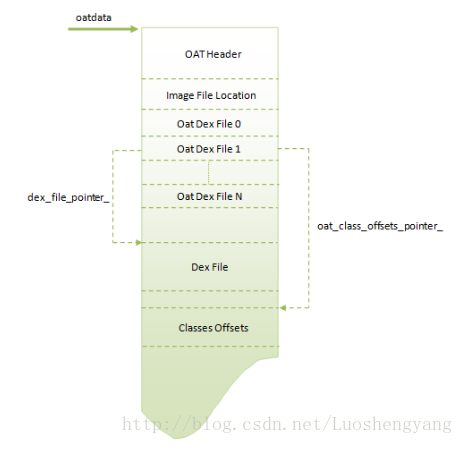
\includegraphics[width=\textwidth]{img/oatdata.png}
\caption{oatdata结构}
\label{fig:oatdata}
\end{figure}

